\chapter{Additional Graphs and Tables}
\section{Simulation}
\begin{table}
	\caption{Ratio of $g^2-1$ of different photon counting schemes to ground truth value  for $\Delta$=1\, pixel/first maximum}
	\begin{tabular}{llllll}
		
		\toprule
		{} &           Raw &        Thres &         Comb &         PSANA &         MaxL \\
		\midrule
		Low Signal  &  12 / 0.6 &  6.9 / 0.6 &  0.6 / 0.8 &   -0.5 / 0.6 &  0.7 / 0.8 \\
		High Signal &    2.4 / 1.0 &  1.8 / 1.0 &  0.7 / 0.8 &  -0.03 / 0.8 &  1.0 / 0.9 \\
		High Noise  &    9.3 / 0.3 &  8.1 / 0.4 &  0.9 / 0.6 &  -0.4 / 0.4 &  0.6 / 0.6 \\
		\bottomrule
	\end{tabular}
\end{table}
\section{Experiment}


\begin{figure}
	\centering
	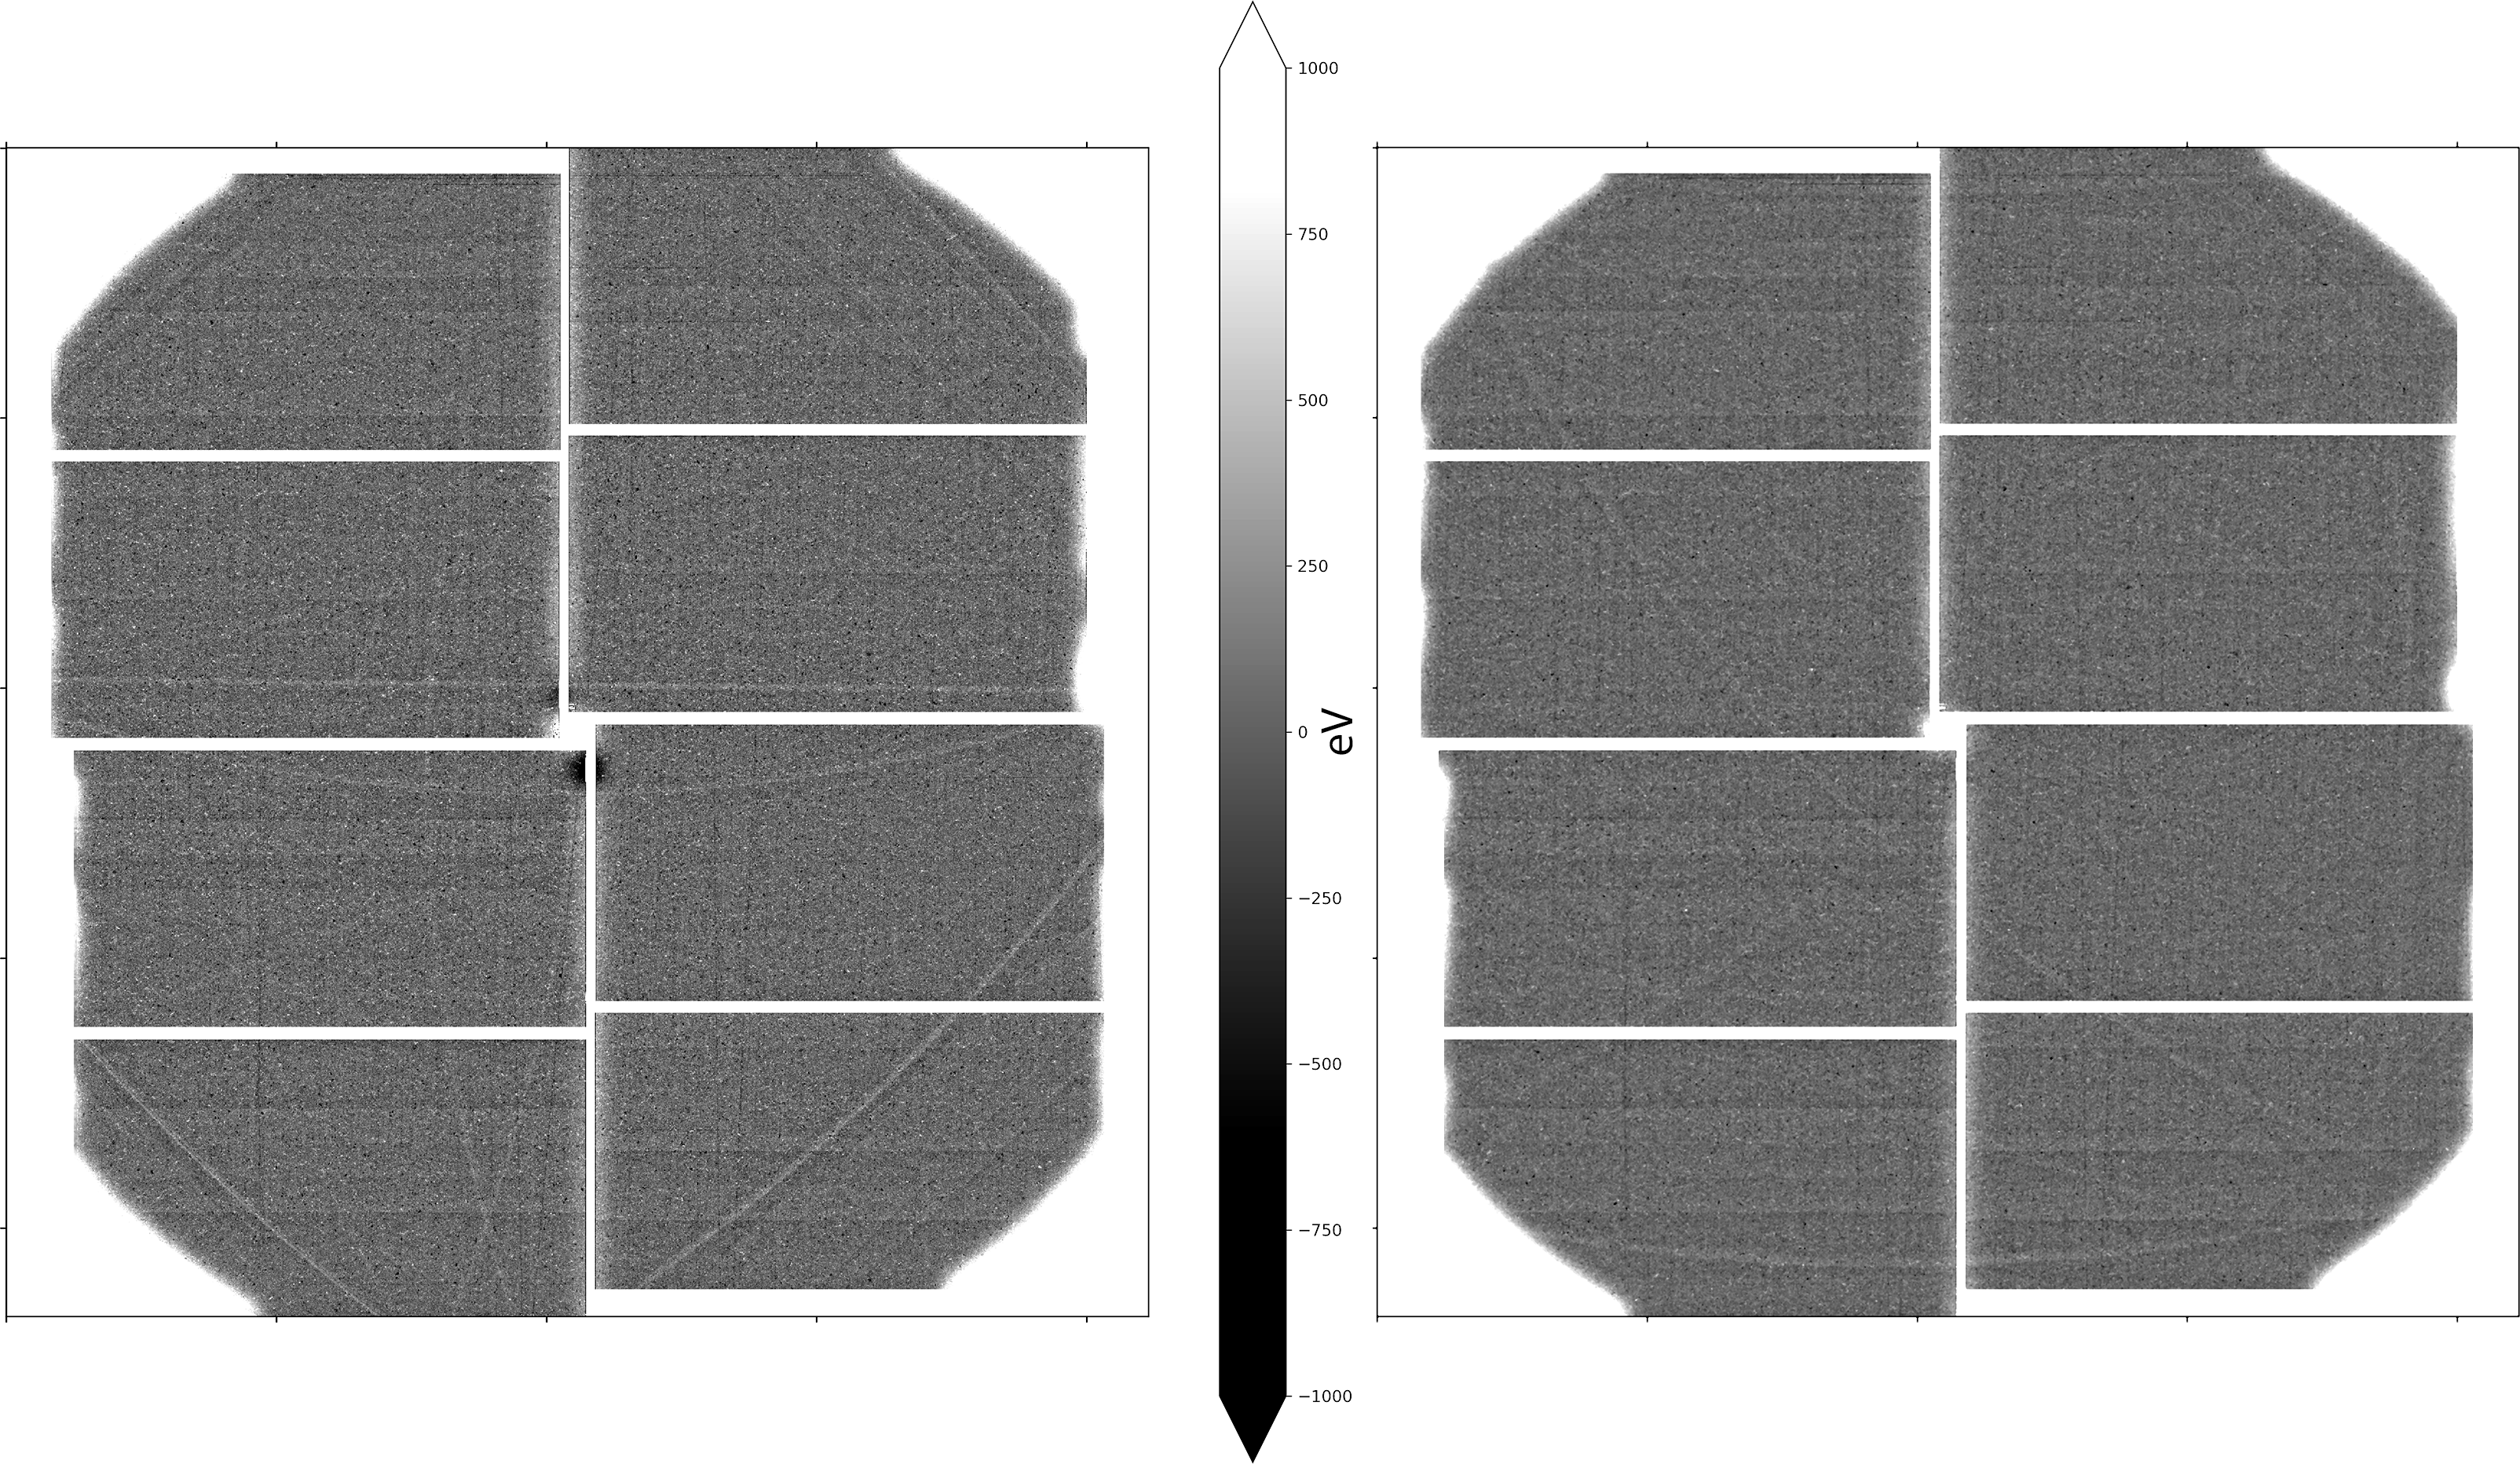
\includegraphics[width=0.8\linewidth]{images/kossel_gaas.png}
	\caption[Mean image of fluorescence of GaAs after background subtraction with visible Kossel lines ]{Mean images of 5000 shots after background subtraction for sample 1 (left) and sample 2 (right), showing the Kossel lines and some artifacts at the edges.}
	\label{fig:kosselgaasmean}
\end{figure}


\begin{table}
	\caption[Miller Indices considered in Kossel line least squares regression of GaAs sample]{Miller Indices considered in Kossel line least squares regression of GaAs sample 1 (left) and sample 2 (right). Not all possible Kossel lines are visible in the recorded images.}
	\begin{tabular}[t]{lll}
		\toprule
		h&           k &        l \\
		\midrule
	 1 & -1 &  1 \\
	-1 &  1 &  1 \\
	-1 & -1 &  1 \\
	2 & -2 &  0 \\
	-2 &  2 &  0 \\
	-2 & -2 &  0 \\
	2 &  2 &  0 \\
	-3 & -1 &  1 \\
	3 &  1 &  1 \\
	-1 & -3 &  1 \\
	2 & -2 &  4 \\
	-2 & -2 &  4 \\
	2 &  2 &  4 \\
	-2 &  2 &  4 \\
	-4 &  0 &  4 \\
	0 &  4 &  4 \\
	4 &  0 &  4 \\
	0 & -4 &  4 \\
				\bottomrule
	\end{tabular}
\hspace{1cm}
	\begin{tabular}[t]{lll}	
	\toprule
	h&           k &        l \\
	\midrule
 2 &  2 &  0 \\
-2 &  2 &  0 \\
2 & -2 &  0 \\
0 & -2 &  2 \\
0 &  2 &  2 \\
2 &  0 &  2 \\
-2 & -2 &  0 \\
-2 &  0 &  2 \\
-3 & -1 &  3 \\
-1 & -3 &  3 \\
1 &  3 &  3 \\
3 &  1 &  3 \\
-1 &  3 &  3 \\
1 & -3 &  3 \\
0 & -4 &  4 \\
-4 &  0 &  4 \\
0 &  4 &  4 \\
4 &  0 &  4 \\
0 &  2 &  6 \\
2 &  0 &  6 \\
-2 &  0 &  6 \\
0 & -2 &  6 \\
	\bottomrule
\end{tabular}
\end{table}